\subsection{Anvendelse af speckle patterns} 
Speckle patterns er et værktøj, som benyttes på tværs af forskellige industrier. Inden for dette projekts relevans kigges der på speckle patterns indenfor mekanik. 

\subsubsection{Digital Image Correlation} Digital image correlation (DIC) er en optisk metode, der anvender digitale billeder til at måle deformation, bevægelse og spændinger i materialer. DIC fungerer ved at sammenligne billeder taget før, under og efter deformation for at bestemme forskydninger og spændingsfelter. Metoden muliggør måling af deformationer uden fysisk kontakt, samt en detaljeret og grundig analyse af materialeegenskaber. (\cite{Zaya2023ApplicationReview})

Fremgangsmetoden for DIC starter med et fotografi taget før belastning (referencebillede), efterfulgt af billeder taget under hele deformationsprocessen (forvredne billeder). Hvert forvredet billede har et unikt tilfældigt speckle pattern sammenlignet med det originale, uforvredne referencebillede. Forskellen mellem referencebilledet og de efterfølgende billeder, kan beregnes ved hjælp af computersoftware ved at sammenkæde alle pixler i referencebilledet, med et hvilket som helst forvredet billede og derefter skabe et spændingsfordelingskort. (\cite{Zaya2023ApplicationReview})

Denne fremgangsmetode viser at DIC-målinger er umulige uden et speckle pattern, da hver prik er med til at dække materialeoverfladen, og dermed indeholder information om deformationen, som er nødvendig for nøjagtig og konsistent sammenligning i den efterfølgende beregning. (\cite{Zaya2023ApplicationReview})

\subsubsection{2D og 3D Digital Image Correlation}
DIC benyttes både til undersøgelser af materialer i planet og i rummet. Til 2D DIC benyttes ét kamera, som tager billeder af materialet. Da der kun benyttes ét kamera, er det kun muligt at undersøge materialet i planet, hvilket kræver at den ønskede overflade er i parallel med kameralinsen. I undersøgelsen må materialet ikke deformere sig ud af planet, da denne bevægelse ikke kan blive set af kameraet. 3D DIC benytter sig af to stereo kameraer og er optimalt i situationer, hvor et materiale bevæger sig fra planet til rummet (figur \ref{fig:2D og 3D DIC}). Stereo kameraer er udstyret med to eller flere linser, som giver mulighed for at tage to  billeder, fra to forskellige små vinkler og kombinere dem til ét billede (her med to linser). Det er også dette menneskeøjet gør, for at give en dybdeopfattelse. Brugen af to stereokameraer gør det muligt at fotografere et objekt fra to forskellige vinkler, og ved hjælp af stereo triangulering, danne en 3D model af objektet. (\cite{Byrne2020DigitalSoftware})

\begin{figure}[H]
    \centering
    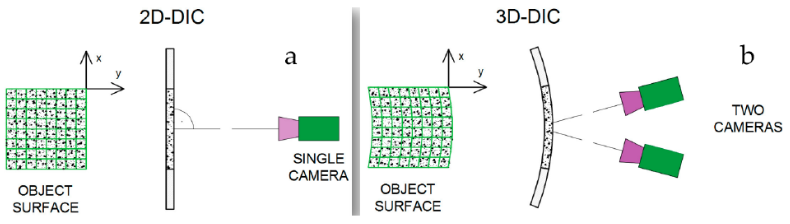
\includegraphics[width=0.9\linewidth]{Sections/2 Problemanalyse/Media/DIC 2D eller 3D.png}
    \caption{Opstilling af 2D og 3D digital image correlation (\cite{Wang2023FiberMonitoring})}
    \label{fig:2D og 3D DIC}
\end{figure}

Vinklen mellem to stereo kameraer og objektet, kaldet stereo vinklen, kan optimeres afhængig af ønsket resultat. Hvis man ønsker større undersøgelse rette mod et plan, kan vinklen mindskes, og til en rumlig undersøgelse, med bevægelse ud af planet, kan vinklen øges. Den optimale stereo vinkel for 3D DIC er mellem 15\degree og 35\degree. (\cite{Bigger2018ACorrelation})


\subsubsection{Speckle pattern til DIC} 
\paragraph{Tykkelse}Det vigtigste for DIC og anvendelse af speckle patterns er om det er kunstigt påført eller naturligt fremkommende. Kunstige speckles vil oftest blive fladt belagt på overfladen (f.eks. ved brug af spraymaling), hvor naturlige speckle patterns, eksempelvis en ru væg, kan variere tykkelsen af prikkerne og forvirre kameraets dybdeopfattelse. Dette kan skabe fejlmålinger og falske spændingsfelter, da kameraet opfanger tykkelsen af prikken, som en del af deformationen, og ikke som målepunkt. Dette gælder både 2D og 3D. (\cite{Byrne2020DigitalSoftware})


%Naturlig speckle patterns opstår ved ruge overflader, her kan dybdeforskelle bruges til at skabe det grey scale. Kunstige speckle patterns er derimod påført efterfølgende. Dette har betydning for opløsningen af analysen.

\paragraph{Materiale}
Siden sin begyndelse i slut 1900-tallet, har DIC gennem årene udviklet sig, og blevet benyttet til en række af forskellige materialeundersøgelser og er blevet til en populær eksperimentel metode blandt andet grundet kosteffektivitet. Materialeundersøgelser som DIC har været igennem inkluderer metaller, polymerer, kompositter, samt biologiske materialer. Disse undersøgelser finder sted på både mikro- og makroskopisk skala, fra millimeter til flere meter. Herved har man også fundet materialer, som ikke er egnet til DIC grundet specifikke faktorer. Nogle af disse inkluderer: Gennemsigtige, bløde eller reflekterende materialer. Løsninger på disse lyder på overfladebelægning af gennemsigtig materiale, benytte speckles af matsort på reflekterende overflader. På bløde materialer er det mere besværligt, men et kamera med en høj rate af billeder i sekundet skal anvendes, grundet skrøbelighed og hurtig deformation. (\cite{Dong2017ACorrelation}; \cite{Bigger2018ACorrelation})


